\newpage
\subsection{Full House}
\label{Full_House}
Wenn in einer Figur 8 Zahlen eingetragen sind, dann kann die Technik \textit{Full House} angewendet werden. Da in jeder Figur die Zahlen 1 bis 9 stehen müssen, kann die fehlende Zahl einfach per Ausschluss ermittelt werden.\\

\begin{figure}[h]
\begin{center}
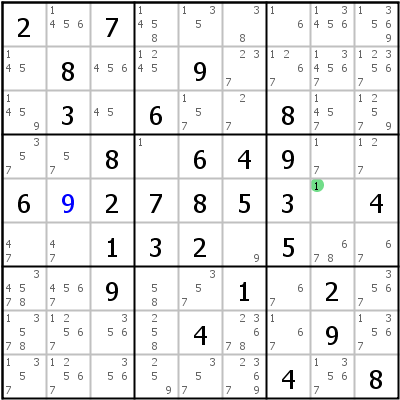
\includegraphics{./img/full_house.png}
\caption{Full House}
\end{center}
\end{figure}

\noindent In \textbf{Abbildung 2.3} fehlt im fünften Block nur noch die Ziffer 2. Alle anderen Ziffern sind bereits in diesem Block eingetragen. Die Sudokuregel besagt, dass in jedem Block die Ziffern 1 bis 9 jeweils einmal vorkommen muss. Daher muss in Zeile 2 Splate 6, im Folgenden z6s6, die Ziffer 2 stehen.